\documentclass[a4paper,12pt]{article}
\usepackage[T1]{fontenc}
\usepackage{fullpage,graphicx,psfrag,amsmath,amsfonts}
\usepackage[small,bf]{caption}
\usepackage[utf8]{inputenc}
\usepackage[english]{babel}
\usepackage{lipsum}
\usepackage{url}
\usepackage{bm}
\usepackage{float}
\usepackage{kpfonts}
\usepackage{mathpazo}
\usepackage{enumitem}
\setitemize{noitemsep,topsep=0pt,parsep=0pt,partopsep=0pt}

\renewcommand*{\a}{\alpha}
\renewcommand*{\t}{\theta}
\renewcommand*{\l}{\ell}
\newcommand*{\T}{^\top}
\newcommand*{\I}{\mathbb{I}}
\newcommand*{\q}{\bm{q}}
\newcommand*{\dotq}{\dot{\q}}
\newcommand*{\de}{\mathop{}\!\mathrm{d}}
\DeclareMathOperator{\sgn}{sgn}

\begin{document}
\author{Filippo Grotto VR460638}

\title{Advanced Control Systems: RPP manipulator}

\maketitle
\tableofcontents

\section{Kinematics}

\subsection{Direct Kinematics}

\begin{center}
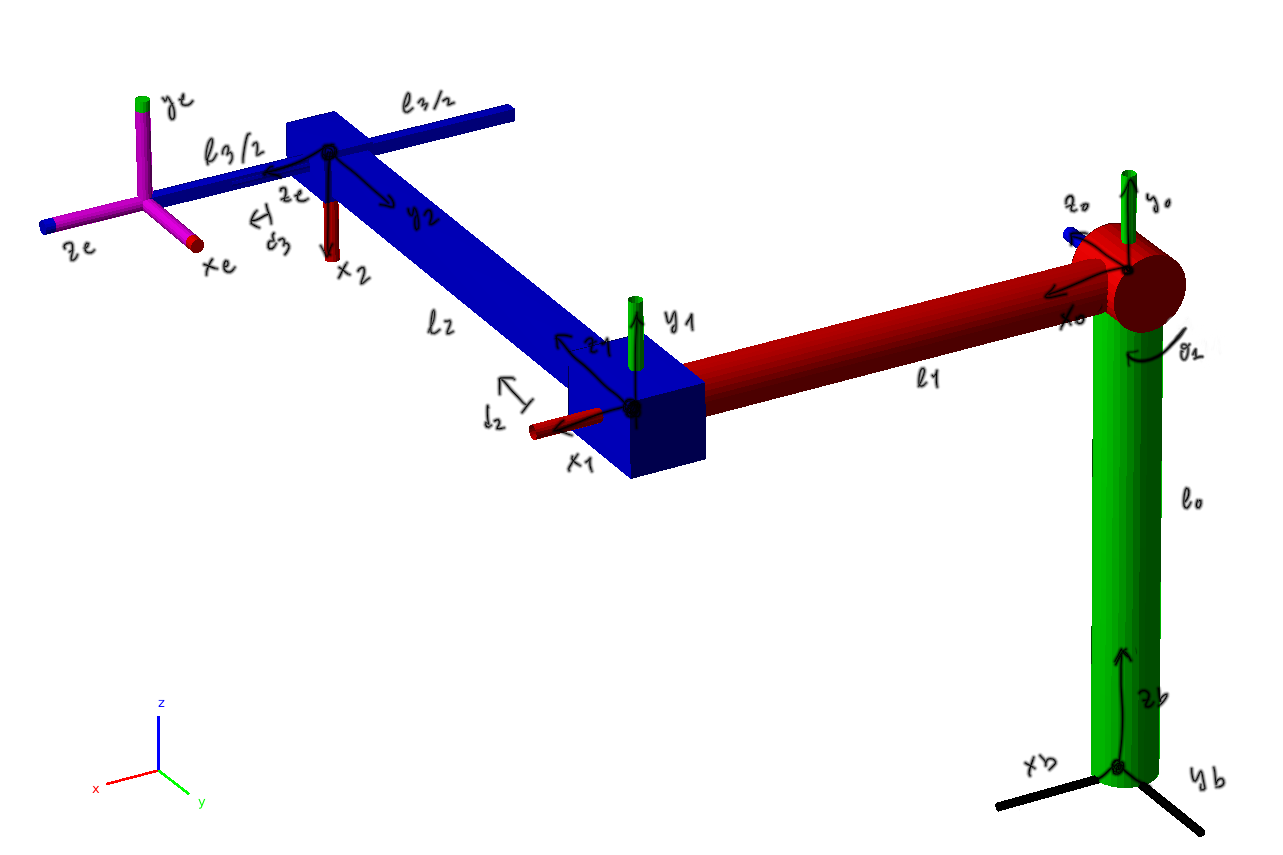
\includegraphics[scale=0.40,trim={10, 10, 10, 10},clip]{images/robot.png}
\end{center}

\noindent Lets define the DH table for our manipulator:

\begin{center}
\begin{tabular}{|c|c|c|c|c|}
    \hline
    $\Sigma_i$ & $d_i$ & $\theta_i$ & $a_i$ & $\alpha_i$ \\ 
    \hline
    $b-0$ & $\l_0$ &    $0$ &    $0$    & $\frac{\pi}{2}$ \\
    $0-1$ &    $0$    & $\t_1$ & $\l_1$ &        $0$ \\
    $1-2$ &    $\l_2+d_2$    & $\frac{\pi}{2}$ & $0$ &        $\frac{\pi}{2}$ \\
    $2-3$ &    $\l_3+d_3$ &    $\frac{\pi}{2}$ &    $0$    &        $0$ \\
    $3-e$ &    $0$    &    $0$ &    $0$    &        $0$ \\
    \hline
\end{tabular}
\end{center}

\noindent The homogenous transformation is defined according to the following matrix and calculated for each row of the DH table. By multiplying $H^b_0H^0_1H^1_2H^2_3H^3_e$ we obtain the final transformation
\[
H^{i - 1}_{i}(q_i) = \begin{bmatrix}
    c_{\t_i} &  - s_{\t_i}c_{\a_i} & s_{\t_i}s_{\a_i} & a_i c_{\t_i} \\
    s_{\t_i} & c_{\t_i}c_{\a_i} &  - c_{\t_i}s_{\a_i} & a_i s_{\t_i} \\
        0    &     s_{\a_i}     &     c_{\a_i}     &     d_i     \\
        0    &         0        &         0        &     1        \\
\end{bmatrix}
\]
\[
H^b_0 = \begin{bmatrix}
    1 & 0 & 0 &    0    \\
    0 & 0 &  - 1 &    0    \\
    0 & 1 & 0 & \l_0 \\
    0 & 0 & 0 &    1    \\
\end{bmatrix}
\qquad
\qquad
H^0_1(\t_1) = \begin{bmatrix}
    c_1 &  - s_1 & 0 & \l_1 c_1 \\
    s_1 & c_1 & 0 & \l_1 s_1 \\
        0    &     0    & 1 &        0        \\
        0    &     0    & 0 &        1        \\
\end{bmatrix}
\qquad
H^1_2(d_2) = \begin{bmatrix}
    0 &  0 & 1 & 0 \\
    1 & 0 & 0 & 0 \\
        0    &    1    & 0 &        d_2+\l_2       \\
        0    &     0    & 0 &        1        \\
\end{bmatrix}
\]
\[
H^2_3(d_3) = \begin{bmatrix}
    0 & -1 & 0 & 0 \\
    1 & 0 & 0 & 0 \\
    0 & 0 & 1 & d_3 + l_3 \\
    0 & 0 & 0 & 1 \\
\end{bmatrix}
\qquad
H^3_e = \begin{bmatrix}
    1 & 0 & 0 & 0 \\
    0 & 1 & 0 & 0 \\
    0 & 0 & 1 & 0 \\
    0 & 0 & 0 & 1 \\
\end{bmatrix}
\]

\[
H^b_e(\q) = \begin{bmatrix}
    0    &  - s_1 & c_1 & c_1(\l_1+\l_3+d_3)\\
    -1   & 0      &  0  &  -\l_2 - d_2 \\
    0    & -c_{1} & s_1 & s_1(\l_1+\l_3+d_3) + \l_0 \\
    0    &     0  & 0   &        1       \\
\end{bmatrix}
\]

\subsection{Inverse Kinematics}
Let's consider the position of ee with respect of the base frame to calculate the value of the joints.
\[
p^b_e = \begin{bmatrix}
    x \\ y \\ z \\
\end{bmatrix}
=
\begin{bmatrix}
    c_1(\l_1+\l_3+d_3)\\
     -\l_2 - d_2 \\
    s_1(\l_1+\l_3+d_3) + \l_0 \\
    1        \\
\end{bmatrix}
\]

It is easy to see that
\[
d_2 = - \l_2 - y \\
\]

\[
\t_1 = \mathop{Atan2}(z-\l_0, x)
\]


For $d_3$ we can apply sum of squares and the result is:
\[
  d_3 = -\l_1 \pm \sqrt{x^2+(z-\l_0)^2} - \l_3  
\]

\section{Jacobians}
\subsection{Geometric Jacobians}
The geometric jacobian is defined as follow with $\q = [\t_1,   d_2,   d_3]^\top$. Note that the matlab robotic toolbox defines the angular velocities above the linear velocities:
\[
\begin{bmatrix}
    \dot{p}_e \\
    \omega_e \\
\end{bmatrix}
 =
\begin{bmatrix}
    \dot{x} \\
    \dot{y} \\
    \dot{z} \\
    \omega_x \\
    \omega_y \\
    \omega_z \\
\end{bmatrix}
 =
\left[
\begin{array}{c|c|c}
    J_{P_1} & J_{P_2} & J_{P_3} \\
    J_{O_1} & J_{O_2} & J_{O_3} \\
\end{array}
\right]
\,
\begin{bmatrix}
    \dot{\t}_1 \\
    \dot{d}_2 \\
    \dot{d}_3 \\
\end{bmatrix}
\]
\begin{align*}
J_{P_1} &= z_0 \times (d^0_e  -  d^0_0) = \begin{bmatrix}
    -s_1(\l_1 + \l_3 + d_3) \\
    0 \\
    c_1(\l_1 + \l_3 + d_3) \\
\end{bmatrix} 
&
J_{O_1} &= z_0 = \begin{bmatrix}0\\0\\1\end{bmatrix}
\\
J_{P_2} &= z_1 = \begin{bmatrix}
     0 \\
     -1 \\
     0 \\
\end{bmatrix} 
&
J_{O_2} &= \begin{bmatrix}0\\0\\0\end{bmatrix}
\\
J_{P_3} &= z_2 = \begin{bmatrix}
    c_1\\
    0\\
    s_1
\end{bmatrix}
&
J_{O_3} &= \begin{bmatrix}0\\0\\0\end{bmatrix}
\end{align*}
We can finally put all the pieces together and obtain the final geometric jacobian:
\[
J(\q) = 
\begin{bmatrix}
    -s_1(\l_1 + \l_3 + d_3) &  0 & c1 \\
     0 &  -1 & 0 \\
     c_1(\l_1 + \l_3 + d_3) & 0 & s1 \\
    0 & 0 & 0 \\
    0 & 0 & 0 \\
    1 & 0 & 0 \\
\end{bmatrix}
\]

\subsection{Analytical Jacobian}
The analytical jacobian can be easily calculated by using partial derivatives of $p^b_e$
\[
p^b_e = \begin{bmatrix}
    x \\ y \\ z \\
\end{bmatrix}
=
\begin{bmatrix}
    c_1(\l_1+\l_3+d_3)\\
     -\l_2 - d_2 \\
    s_1(\l_1+\l_3+d_3) + \l_0 \\
    1        \\
\end{bmatrix}
\]

\noindent Finally we end up with the analytical jacobian
\[
Ja(\q) = 
\begin{bmatrix}
    -s_1(\l_1 + \l_3 + d_3) &  0 & c1 \\
     0 &  -1 & 0 \\
     c_1(\l_1 + \l_3 + d_3) & 0 & s1 \\
    1 & 0 & 0 \\
    0 & 0 & 0 \\
    0 & 0 & 0 \\
\end{bmatrix}
\]

\noindent Another possibility is to use the relation between the geometric and analytical jacobian as follow using ZYZ:

\[
\omega_e = T(\phi_e)\dot{\phi}_e
\qquad
T(\phi_e) = \begin{bmatrix}
    0 & -s_\varphi & c_\varphi s_\theta \\
    0 &  c_\varphi & s_\varphi s_\theta \\
    1 &          0 &           c_\theta \\
\end{bmatrix}
\]

\[
J(\q) = T_A(\phi_e) J_A(\q)
\]
\[
T_A(\phi_e) = \begin{bmatrix}
    \I_3 & \emptyset_3 \\ 
\emptyset_3 &     T(\phi_e) \\
\end{bmatrix}
\]

\section{Energy}
Let's calculate $p_{\l_i}$ of the center of mass wrt of $\Sigma_0$. To get them let's calculate $p^i_{\l_i}$ of the center of mass wrt of $\Sigma_i$
\[
p_{\l_1}^{1} = \begin{bmatrix}  - \frac{\l_1}{2} \\ 0 \\ 0 \end{bmatrix}
\qquad
\qquad
p_{\l_2}^{2} = \begin{bmatrix} 0 \\ 0 \\  - \frac{\l_2}{2} \end{bmatrix}
\qquad
\qquad
p_{\l_3}^{3} = \begin{bmatrix} 0 \\ 0 \\  - \frac{\l_3}{2} \end{bmatrix}
\]
we can express the homogenous wrt of $\Sigma_0$ using the following formula: 
\[
p_{\l_i} = R^0_i p_{\l_i}^{i}  +  d^0_i
\] 

\subsection{Potential Energy}
The potential energy is calculated according to the formula:
\[
    U_i = -m_{l_i}g_0^{T}p_{l_i}
    \qquad
    g_0 = \begin{bmatrix}
        0\\ 0 \\ -g
    \end{bmatrix}
\]
\noindent The total potential energy is the sum of the 3 contributions $U_1$ $U_2$ and $U_3$. The total expression is reported and was calculated using the MATLAB symbolic toolbox ($L_{ih}$ is the length of i-th link and $m_i$ is the mass)
\[
    U = \frac{-gsin(\theta_1)(L_{1h}m_1 + 2L_{1h}m_2 + 2L_{1h}m_3 + L_{3h}m_3 + 2d_3m_3)}{2}  
\]

\subsection{Kinetic Energy}
The kinetic energy is calculated using the following formula:
\[
\mathcal{T}(\q,\dotq) = \frac{1}{2}\dotq\T B(\q) \dotq
\]

\[
B(\q) = \sum_{i=1}^{n} B_i(\q)
      = \sum_{i=1}^{n} m_{\l_i} \bigl({J^{\l_i}_{P}}\T J^{\l_i}_{P}\bigr)
       +  \bigl({R_i^0}\T J^{\l_i}_{O}\bigr)\T I_{\l_i}^{i} \bigl({R_i^0}\T J^{\l_i}_{O}\bigr)
\]

\noindent It is necessary to calculate the inertia tensors $I_{\l_i}^{i}$ and the partial jacobians $J^{\l_i}_{P}$ and $J^{\l_i}_{O}$. We will use the steiner theorem because all frames $\Sigma_i$ are translated of $p_{\l_i}^{i}$ w.r.t. of the center of mass (i.e inertia tensor w.r.t. of the axis of the joint that the
link is attached).
\[
    I_{\l_1}^{1} = I_{\l_1}^{C_1} + m_{\l_1}S^{T}(r)S(r) = I_{\l_1}^{C_1}  +  m_{\l_1}\bigl(r\T r \I_{3,3}  -  r r\T\bigr) 
\]
For the inertia tensors we can use the following formulas for the cylindrical and prismatic links considering that the prismatic links have a square base.
\[
    I^C_{cylinder} = \frac{1}{2}\begin{bmatrix}
        m(a^2+b^2) & 0 &0 \\
        0 &m(3(a^2+b^2)^2+h^2)& 0 \\
        0& 0& m(3(a^2+b^2)^2+h^2)
    \end{bmatrix}
\]

\[
    I^C_{prismatic} = \frac{1}{12}\begin{bmatrix}
        m(b^2+c^2) & 0 &0 \\
        0 &m(a^2+c^2)^2& 0 \\
        0& 0& m(a^2+b^2)
    \end{bmatrix}
\]

\bigskip
\noindent Finally we need to compute the partial jacobians in order to calculate velocity of intermediate links.

\[
    J^{\l_i}_{P_j} = \begin{cases}
       z_{j-1} & \text{prismatic joint} \\
       z_{j-1} \times (p_{l_i}- p_{j-1}) & \text{revolute joint} 
      \end{cases}
    \qquad
    J^{\l_i}_{O_j} = \begin{cases}
    0 & \text{prismatic joint} \\
    z_{j-1} & \text{revolute joint} 
    \end{cases}
\]

\noindent In our case the computer partial jacobians are:

\[
    J^{\l_1}_{P} = \begin{bmatrix}
        -\l_1sin(\theta_1)/2 & 0 & 0 \\
 \l_1cos(\theta_1)/2 &0 &0 \\
               0 &0 &0
    \end{bmatrix}
    \qquad
    J^{\l_2}_{P} = \begin{bmatrix}
        \l_2cos(\theta_1)/2 - \l_1sin(\theta_1) &0 &0\\
\l_1cos(\theta_1) + (\l_2sin(\theta_1))/2& 0 &0\\
                            0& 1& 0;
    \end{bmatrix}
\]
\[
    J^{\l_3}_{P} = \begin{bmatrix}
        -sin(\theta_1)(\l_1 + \l_3h/2 + d_3) &0 & cos(\theta_1)\\
 cos(\theta_1)(\l_1 + \l_3h/2 + d_3) &0 &sin(\theta_1)\\
                          0 &1 &      0
    \end{bmatrix}
    \qquad
    J^{\l_1}_{O_j} = J^{\l_2}_{O_j} = J^{\l_3}_{O_j} =\begin{bmatrix}
        0 &0 &0\\ 0& 0 &0\\ 1& 0& 0
    \end{bmatrix}
\]

\[
  B(\textbf{q}) = B_1(\textbf{q}) + B_2(\textbf{q}) +B_3(\textbf{q}) 
\]

\noindent Finally we can recover the kinetic energy using the calculated $B(\textbf{q})$ and $ \dot{\textbf{q}}$.
\end{document}